% Metódy inžinierskej práce

\documentclass{coursepaper}

\usepackage[slovak]{babel}
\usepackage[IL2]{fontenc} % lepšia sadzba písmena Ľ než v T1
\usepackage[utf8]{inputenc}
\usepackage{graphicx}
\usepackage{url} % príkaz \url na formátovanie URL
\usepackage{hyperref} % odkazy v texte budú aktívne
% ===== Grafika a PDF =====
\usepackage{graphicx}
\usepackage{pdfpages}            % vloženie PDF
\usepackage{hyperref} 

\usepackage{cite}


\pagestyle{headings}

\title{Názov\thanks{Semestrálny projekt v predmete Metódy inžinierskej práce, ak. rok 2015/16, vedenie: Meno Priezvisko}}

\author{Yaroalav Nesteruk\\[2pt]
	{\small Slovenská technická univerzita v Bratislave}\\
	{\small Fakulta informatiky a informačných technológií}\\
	{\small \texttt{...@stuba.sk}}
	}

\date{\small 07. oktober 2025}

\begin{document}
\maketitle


\section{Úvod}
Umelá inteligencia (AI) sa stala jednou z najdynamickejšie sa rozvíjajúcich oblastí informatiky. Jej vplyv siaha od priemyslu až po každodenný život. Cieľom tejto ohladovej štúdie je zhrnúť základné princípy, metódy a smerovanie moderného výskumu v tejto oblasti.

\section{Ciele práce}
Cieľom práce je analyzovať aktuálne trendy v oblasti umelej inteligencie a poukázať na ich praktické uplatnenie v rôznych odvetviach – od medicíny po dopravu.

\section{Použité metódy}
Pri spracovaní článku boli použité metódy analýzy odborných publikácií, štatistické porovnanie výsledkov experimentov a syntéza poznatkov z viacerých zdrojov.

\section{Výsledky a diskusia}
Na základe štúdia relevantných zdrojov možno pozorovať, že najrýchlejší rozvoj nastáva v oblastiach neurónových sietí a generatívnych modelov. Veľkú pozornosť si zaslúži aj oblasť etiky AI – otázky súkromia, zaujatosti a transparentnosti algoritmov.

% ===== Vloženie PDF =====
\section{Príloha PDF}
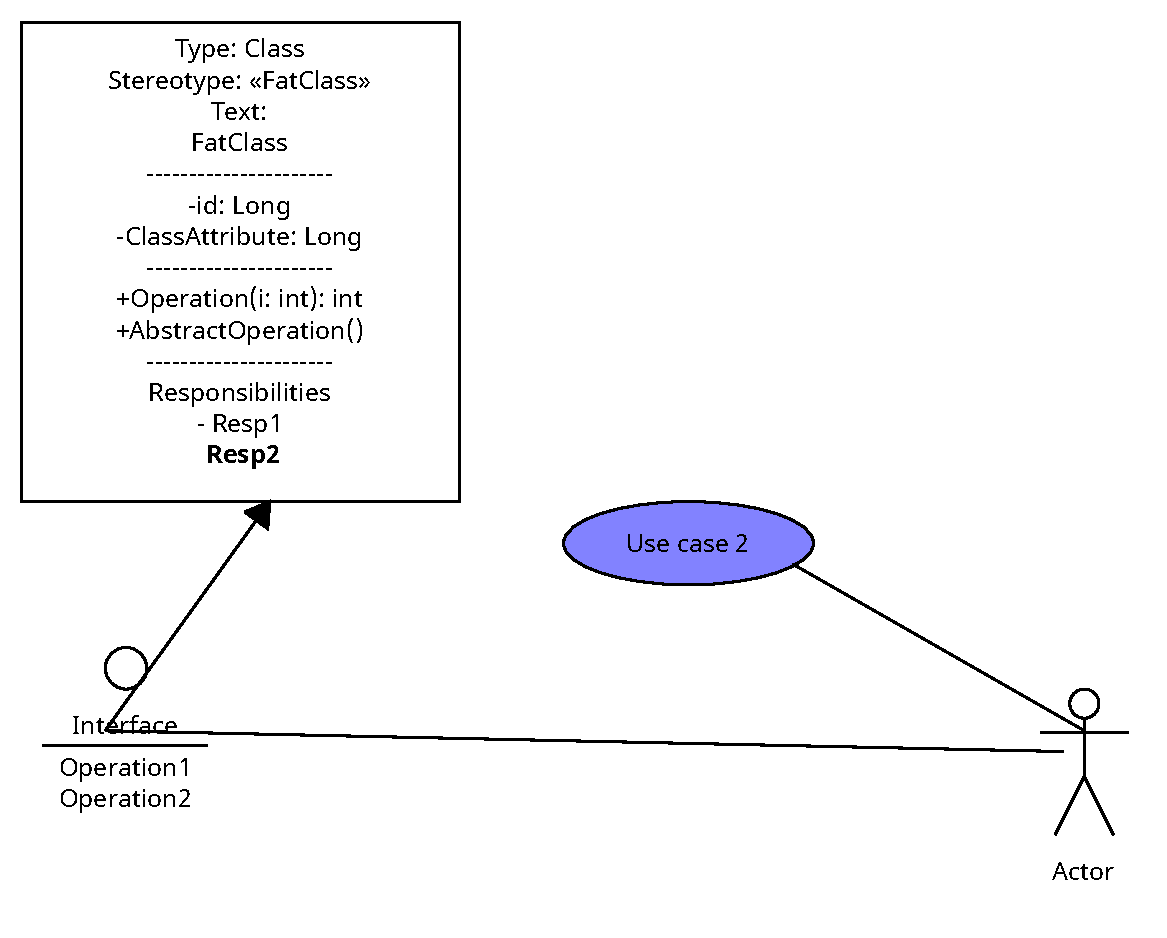
\includepdf[pages=-]{nieco.pdf}  % vloží všetky strany PDF

\section{Záver}
Umelá inteligencia bude v nasledujúcich rokoch zohrávať kľúčovú úlohu vo všetkých sférach spoločnosti. Preto je potrebné venovať pozornosť nielen technickému rozvoju, ale aj spoločenským dopadom tejto technológie.

\section{Literatúra}
\begin{thebibliography}{9}
\bibitem{Goodfellow2016}
Ian Goodfellow, Yoshua Bengio, Aaron Courville. \emph{Deep Learning}. MIT Press, 2016.

\bibitem{Russell2010}
Stuart Russell, Peter Norvig. \emph{Artificial Intelligence: A Modern Approach}. Pearson, 2010.

\bibitem{EthicsAI2021}
Floridi, L. a kol. \emph{Ethics of Artificial Intelligence: Principles and Practice}. Oxford University Press, 2021.
\end{thebibliography}

%\acknowledgement{Ak niekomu chcete poďakovať\ldots}

\bibliography{literatura}
\bibliographystyle{alpha}
\end{document}

